\chapter{Interview Summary with IT Staff}\label{app:appendix_interview}

This appendix presents the summary of an interview conducted face-to-face with a university IT staff member on Monday, June 2, 2025. The interview aimed to validate and support the technical aspects of the research, especially in terms of log management and forensic readiness related to online examinations using Moodle.

\section*{Question 1}
\textbf{How does the team respond to cheating incidents such as impersonation (jockeying)?}

\begin{itemize}
	\item \textbf{Method:} Currently, the LAC team uses several indicators, such as identical values or patterns in quiz attempts. Monitoring is also done via Zoom, where suspicious behavior like continuous question reading or remote cursor movement can indicate possible impersonation.
	\item \textbf{Challenges:} SEB uses a predefined application blacklist, but it is difficult to block portable applications that are not installed. 
	\item \textbf{Output:} The hope is to create more sophisticated device-level restrictions to prevent such cheating tactics.
\end{itemize}

\section*{Question 2}
\textbf{What log sources are typically identified (firewall, server, endpoint, application, etc.)?}

\begin{itemize}
	\item \textbf{Method:} Currently, the system is integrated with Cloudflare for proxy and firewall at both the application and database layers. Zoom recording logs are also used for additional evidence. Web server logs and user-agent strings are checked from Cloudflare.
	\item \textbf{Challenges:} VPN usage is a concern. Although some regional restrictions are in place, forensics becomes more complex due to these circumventions.
	\item \textbf{Output:} The goal is to produce forensic reports that can be understood by non-IT stakeholders for decision-making, such as determining if students should retake the exam.
\end{itemize}

\section*{Question 3}
\textbf{How is log data collected to detect cheating attempts?}

\begin{itemize}
	\item \textbf{Method:} Log data is collected manually. For application logs, the team accesses Moodle quiz and course logs. For database logs, standard general logs are used, and quiz attempt data requires querying multiple tables.
	\item \textbf{Challenges:} The volume of log data is large and growing. As a result, the current process is reactive. Log retention policies are as follows: quiz attempt logs are retained for 3 days, application/database logs for 2 years, and Cloudflare logs for 7 days. Due to Moodle–iGracias integration, quiz logs are only retained for 1 day.
	\item \textbf{Output:} There is a need to centralize log storage and retrieval.
\end{itemize}

\section*{Question 4}
\textbf{How does the team determine which logs are relevant for security and incidents?}

\begin{itemize}
	\item \textbf{Method:} Database logs are used to trace user activity, including quiz start and end times. Web service logs and Cloudflare logs are used for additional verification.
	\item \textbf{Challenges:} Identifying the right query formulas is essential. Translating technical logs into understandable formats for non-IT decision-makers is a major challenge.
	\item \textbf{Output:} Reports are provided in Excel format, including exam schedules, login activity, IP addresses, devices, locations, quiz navigation, and exam states per page, along with timing details.
\end{itemize}

\section*{Question 5}
\textbf{Are logs collected in real-time or periodically? If periodic, what is the interval?}

\begin{itemize}
	\item \textbf{Method:} Logs are collected on-demand based on LAC requests.
	\item \textbf{Challenges:} Time gaps in collection cause log loss. Querying large datasets increases database server load. Zipping logs during exams may result in missing entries. VMSS auto-destroy policies cause Apache/PHP logs to be lost.
	\item \textbf{Output:} The goal is to shift to a proactive, scheduled log collection system.
\end{itemize}

\section*{Question 6}
\textbf{How long are logs stored, and is there a log retention policy?}

\begin{itemize}
	\item \textbf{Method:} Logs in Celoe are retained for 2 years. In LAC, logs are deleted one day after the exam (H+1).
	\item \textbf{Challenges:} Data volume is increasing rapidly.
	\item \textbf{Output:} There is a need to evaluate log retention efficiency and develop a policy aligned with storage capacity.
\end{itemize}

\section*{Question 7}
\textbf{What is the log storage mechanism (on-premise/cloud, encrypted/not)?}

\begin{itemize}
	\item \textbf{Method:} Apache and web service logs are stored in cloud-based VM storage. Database logs are also stored in cloud-based VMs.
	\item \textbf{Challenges:} Multi-instance architecture requires mapping volumes using NFS. Logs are synced using \texttt{rsync} every minute, which causes data duplication and bloated storage usage.
	\item \textbf{Output:} The team hopes for more centralized log management. Compression reduces storage size but increases CPU usage due to high zipping overhead.
\end{itemize}

\section*{Question 8}
\textbf{Is there a log backup mechanism for forensic purposes?}

\begin{itemize}
	\item \textbf{Method:} Logs are backed up, but forensic procedures have not been formally implemented. Currently, log retrieval is manual.
	\item \textbf{Challenges:} There is no dedicated forensic team. Most decisions are made by the Celoe team with support from LAC.
	\item \textbf{Output:} Moving toward centralized log collection would enhance forensic capability, which is currently very limited.
\end{itemize}
% \chapter{MISCELLANEOUS}\label{app:appendix_A}
% This chapter discusses how to insert equation, figure and table on \LaTeX~document. All the object in this chapter just the examples to make you ease to write your awesome thesis.
% \section{Equation \#examples}
% For simple equation, There is a equation $10 + 5x=0$, then determine the value of x by solving that algebraic equation problem. The answer is shown by equation \ref{eq:plus}
% 	\begin{equation}
% 		\label{eq:plus}
% 			\begin{aligned}
% 			10 + 5x = 0 \\
% 			5x = -10\\
% 			x = -2\\
% 		\end{aligned}
% 	\end{equation}
% Besides that, for complicated equation will be explained as follow. The general equation for a 2D ($N$ by $M$ image) Discrete Cosine Transform is defined by equation \ref{eq:dct}
% 	\begin{equation}
% 	\label{eq:dct}
% 		F(u,v)=\sqrt{\frac{2}{N}} \sqrt{\frac{2}{M}} \sum_{i=0}^{N-1} A(i)*\cos \left(\frac{u(2i+1)\pi}{2N}\right)*\sum_{j=0}^{M-1} A(j)*\cos \left(\frac{v(2j+1)\pi}{2M}\right)*f(i,j)
% 	\end{equation}
% where $A(i)$ is defined as $\left\{ \begin{aligned} \frac{1}{\sqrt{2}}~,~for~u~=~0\\1~,~otherwise \end{aligned} \right.$, while $A(j)$ as $\left\{ \begin{aligned} \frac{1}{\sqrt{2}}~,~for~v~=~0\\1~,~otherwise \end{aligned} \right.$

% \section{Figure \#examples}
% This section contain how to insert figure (see figure \ref{fig:digital}) and block diagram (see figure \ref{blo:biometrics}). We recommend to use high resolution JPEG or JPG instead PNG format, it will make the compiling process to PDF faster, size of the PDF file is smaller and the quality is image still better when the PDF is print out or zooming out.
% 	\begin{figure}[H]
% 		\centering
% 		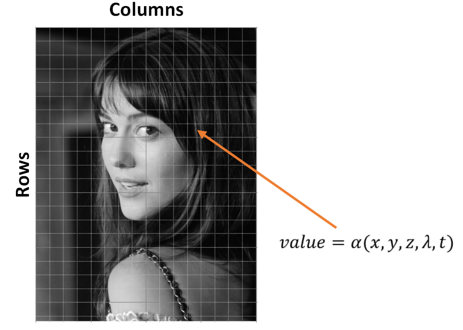
\includegraphics[width=2.5in]{figure/fig_digital}
% 		\caption{Picture of mary elizabeth winstead}
% 		\label{fig:digital}
% 	\end{figure}	
% 	\begin{figure}[H]
% 		\centering
% 		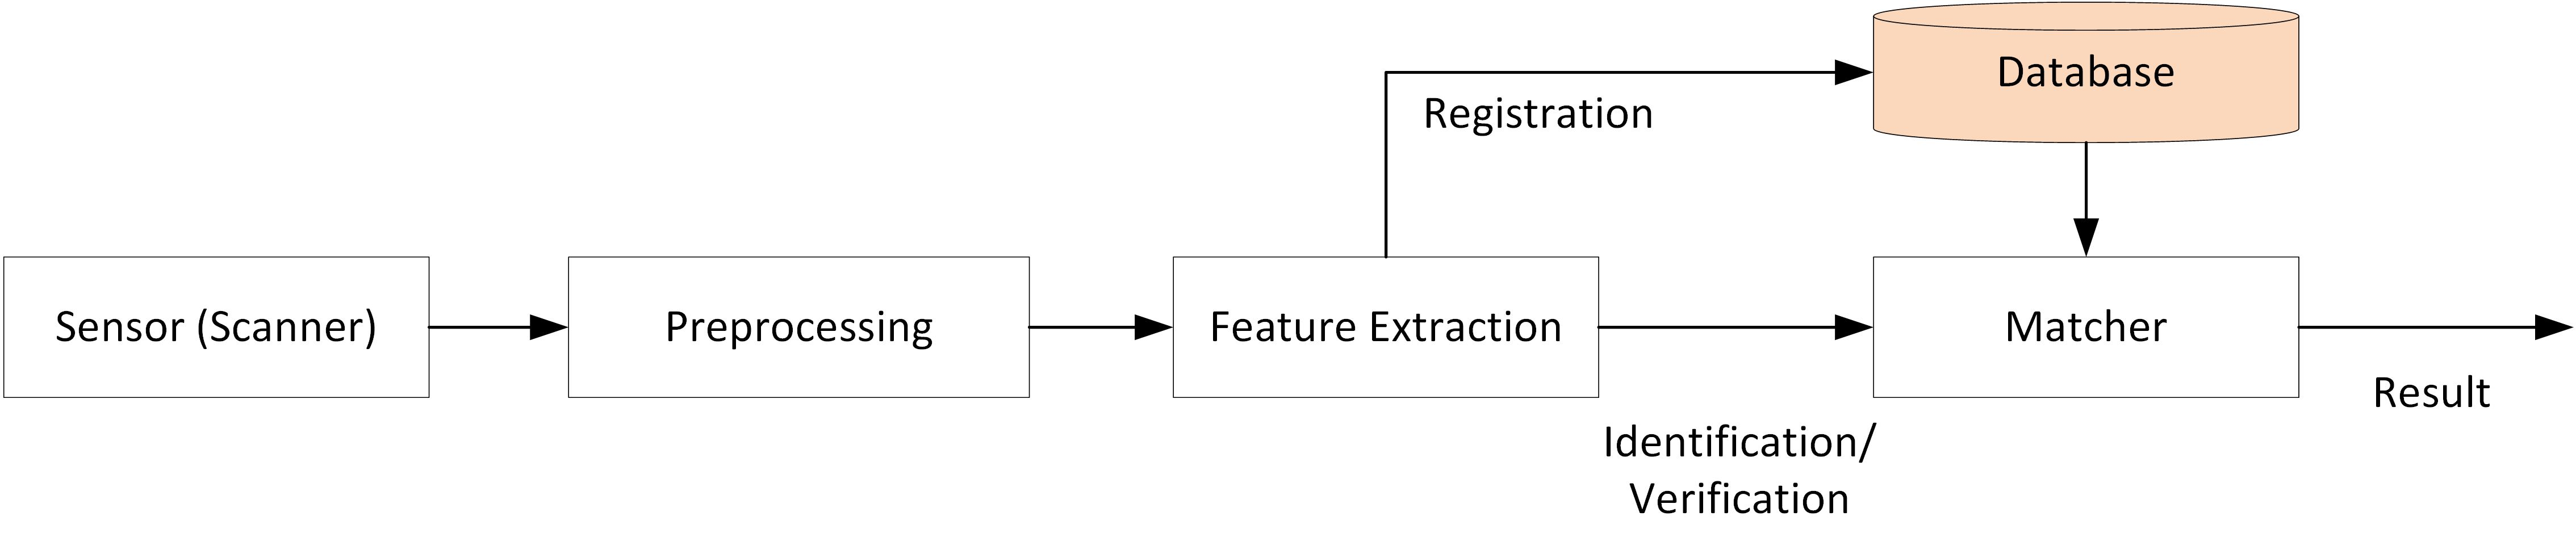
\includegraphics[width=5.5in]{block/gen_biometrics}
% 		\caption{Example of block diagram.}
% 		\label{blo:biometrics}
% 	\end{figure}	
	
% \section{Table \#examples}
% The regular table (see table \ref{tab:simpleTab}) only can be used in single page. So, for the long table which use multiple pages is recommended to use longtable (see table \ref{tab:fisher_irish})
% \begin{enumerate}
% 	\item Table\\
% 	Table \ref{tab:simpleTab} will show you how to cite the reference, it can be the author or the year of the reference.
% 		\begin{table}[H]
% 		  \centering \caption{Example of Tables}
% 			\begin{tabular}{|p{1.5cm}|p{3.5cm}|p{3.5cm}|}
% 			\hline
% 			\multicolumn{1}{|c|}{\textbf{Reference}} & \multicolumn{2}{c|}{\textbf{Paper or Journal}} \\
% 			\cline{2-3}    \multicolumn{1}{|c|}{} & \multicolumn{1}{c|}{\textit{\textbf{Authors}}} & \multicolumn{1}{c|}{\textit{\textbf{Full Authors}}} \\
% 			\hline
% 			\cite{01_journal} & \citet{01_journal}$^a$ & \citefullauthor{01_journal} \\
% 			\hline
% 			\cite{02_journal} & \citet{02_journal} & \citefullauthor{02_journal} \\
% 			\hline
% 			\cite{03_journal} & \citet{03_journal} & \citefullauthor{03_journal} \\
% 			\hline
% 			\cite{04_journal} & \citet{04_journal} & \citefullauthor{04_journal} \\
% 			\hline
% 			\multicolumn{3}{l}{
% 				\begin{footnotesize}
% 					$^a$ : \citeyear{01_journal}.********.
% 				\end{footnotesize}
% 			} \\
% 			\end{tabular}%
% 		  \label{tab:simpleTab}%
% 		\end{table}%
% 	\item Longtable
% 		\begin{center}
% 			\begin{longtable}{|r|r|r|r|r|}\caption{Iris flower data set \#Example of longtable}\label{tab:fisher_irish}\\
% 				\hline
% 				\textbf{Sepal length} & \textbf{Sepal width} & \textbf{Petal length} & \textbf{Petal width} & \textbf{Species} \\
% 				\hline
% 				\endfirsthead
% 				\hline
% 				\textbf{Sepal length} & \textbf{Sepal width} & \textbf{Petal length} & \textbf{Petal width} & \textbf{Species} \\
% 				\hline
% 				\endhead
% 				5.1   & 3.5   & 1.4   & 0.2   & \textit{I. setosa} \\
% 				\hline
% 				4.9   & 3     & 1.4   & 0.2   & \textit{I. setosa} \\
% 				\hline
% 				4.7   & 3.2   & 1.3   & 0.2   & \textit{I. setosa} \\
% 				\hline
% 				4.6   & 3.1   & 1.5   & 0.2   & \textit{I. setosa} \\
% 				\hline
% 				5     & 3.6   & 1.4   & 0.2   & \textit{I. setosa} \\
% 				\hline
% 				5.4   & 3.9   & 1.7   & 0.4   & \textit{I. setosa} \\
% 				\hline
% 				4.6   & 3.4   & 1.4   & 0.3   & \textit{I. setosa} \\
% 				\hline
% 				5     & 3.4   & 1.5   & 0.2   & \textit{I. setosa} \\
% 				\hline
% 				4.4   & 2.9   & 1.4   & 0.2   & \textit{I. setosa} \\
% 				\hline
% 				4.9   & 3.1   & 1.5   & 0.1   & \textit{I. setosa} \\
% 				\hline
% 				5.4   & 3.7   & 1.5   & 0.2   & \textit{I. setosa} \\
% 				\hline
% 				4.8   & 3.4   & 1.6   & 0.2   & \textit{I. setosa} \\
% 				\hline
% 				4.8   & 3     & 1.4   & 0.1   & \textit{I. setosa} \\
% 				\hline
% 				4.3   & 3     & 1.1   & 0.1   & \textit{I. setosa} \\
% 				\hline
% 				5.8   & 4     & 1.2   & 0.2   & \textit{I. setosa} \\
% 				\hline
% 				5.7   & 4.4   & 1.5   & 0.4   & \textit{I. setosa} \\
% 				\hline
% 				5.4   & 3.9   & 1.3   & 0.4   & \textit{I. setosa} \\
% 				\hline
% 				5.1   & 3.5   & 1.4   & 0.3   & \textit{I. setosa} \\
% 				\hline
% 				5.7   & 3.8   & 1.7   & 0.3   & \textit{I. setosa} \\
% 				\hline
% 				5.1   & 3.8   & 1.5   & 0.3   & \textit{I. setosa} \\
% 				\hline
% 				5.4   & 3.4   & 1.7   & 0.2   & \textit{I. setosa} \\
% 				\hline
% 				5.1   & 3.7   & 1.5   & 0.4   & \textit{I. setosa} \\
% 				\hline
% 				4.6   & 3.6   & 1     & 0.2   & \textit{I. setosa} \\
% 				\hline
% 				5.1   & 3.3   & 1.7   & 0.5   & \textit{I. setosa} \\
% 				\hline
% 				4.8   & 3.4   & 1.9   & 0.2   & \textit{I. setosa} \\
% 				\hline
% 				5     & 3     & 1.6   & 0.2   & \textit{I. setosa} \\
% 				\hline
% 				5     & 3.4   & 1.6   & 0.4   & \textit{I. setosa} \\
% 				\hline
% 				5.2   & 3.5   & 1.5   & 0.2   & \textit{I. setosa} \\
% 				\hline
% 				5.2   & 3.4   & 1.4   & 0.2   & \textit{I. setosa} \\
% 				\hline
% 				4.7   & 3.2   & 1.6   & 0.2   & \textit{I. setosa} \\
% 				\hline
% 				4.8   & 3.1   & 1.6   & 0.2   & \textit{I. setosa} \\
% 				\hline
% 				5.4   & 3.4   & 1.5   & 0.4   & \textit{I. setosa} \\
% 				\hline
% 				5.2   & 4.1   & 1.5   & 0.1   & \textit{I. setosa} \\
% 				\hline
% 				5.5   & 4.2   & 1.4   & 0.2   & \textit{I. setosa} \\
% 				\hline
% 				4.9   & 3.1   & 1.5   & 0.2   & \textit{I. setosa} \\
% 				\hline
% 				5     & 3.2   & 1.2   & 0.2   & \textit{I. setosa} \\
% 				\hline
% 				5.5   & 3.5   & 1.3   & 0.2   & \textit{I. setosa} \\
% 				\hline
% 				4.9   & 3.6   & 1.4   & 0.1   & \textit{I. setosa} \\
% 				\hline
% 				4.4   & 3     & 1.3   & 0.2   & \textit{I. setosa} \\
% 				\hline
% 				5.1   & 3.4   & 1.5   & 0.2   & \textit{I. setosa} \\
% 				\hline
% 				5     & 3.5   & 1.3   & 0.3   & \textit{I. setosa} \\
% 				\hline
% 				4.5   & 2.3   & 1.3   & 0.3   & \textit{I. setosa} \\
% 				\hline
% 				4.4   & 3.2   & 1.3   & 0.2   & \textit{I. setosa} \\
% 				\hline
% 				5     & 3.5   & 1.6   & 0.6   & \textit{I. setosa} \\
% 				\hline
% 				5.1   & 3.8   & 1.9   & 0.4   & \textit{I. setosa} \\
% 				\hline
% 				4.8   & 3     & 1.4   & 0.3   & \textit{I. setosa} \\
% 				\hline
% 				5.1   & 3.8   & 1.6   & 0.2   & \textit{I. setosa} \\
% 				\hline
% 				4.6   & 3.2   & 1.4   & 0.2   & \textit{I. setosa} \\
% 				\hline
% 				5.3   & 3.7   & 1.5   & 0.2   & \textit{I. setosa} \\
% 				\hline
% 				5     & 3.3   & 1.4   & 0.2   & \textit{I. setosa} \\
% 				\hline
% 				7     & 3.2   & 4.7   & 1.4   & \textit{I. versicolor} \\
% 				\hline
% 				6.4   & 3.2   & 4.5   & 1.5   & \textit{I. versicolor} \\
% 				\hline
% 				6.9   & 3.1   & 4.9   & 1.5   & \textit{I. versicolor} \\
% 				\hline
% 				5.5   & 2.3   & 4     & 1.3   & \textit{I. versicolor} \\
% 				\hline
% 				6.5   & 2.8   & 4.6   & 1.5   & \textit{I. versicolor} \\
% 				\hline
% 				5.7   & 2.8   & 4.5   & 1.3   & \textit{I. versicolor} \\
% 				\hline
% 				6.3   & 3.3   & 4.7   & 1.6   & \textit{I. versicolor} \\
% 				\hline
% 				4.9   & 2.4   & 3.3   & 1     & \textit{I. versicolor} \\
% 				\hline
% 				6.6   & 2.9   & 4.6   & 1.3   & \textit{I. versicolor} \\
% 				\hline
% 				5.2   & 2.7   & 3.9   & 1.4   & \textit{I. versicolor} \\
% 				\hline
% 				5     & 2     & 3.5   & 1     & \textit{I. versicolor} \\
% 				\hline
% 				5.9   & 3     & 4.2   & 1.5   & \textit{I. versicolor} \\
% 				\hline
% 				6     & 2.2   & 4     & 1     & \textit{I. versicolor} \\
% 				\hline
% 				6.1   & 2.9   & 4.7   & 1.4   & \textit{I. versicolor} \\
% 				\hline
% 				5.6   & 2.9   & 3.6   & 1.3   & \textit{I. versicolor} \\
% 				\hline
% 				6.7   & 3.1   & 4.4   & 1.4   & \textit{I. versicolor} \\
% 				\hline
% 				5.6   & 3     & 4.5   & 1.5   & \textit{I. versicolor} \\
% 				\hline
% 				5.8   & 2.7   & 4.1   & 1     & \textit{I. versicolor} \\
% 				\hline
% 				6.2   & 2.2   & 4.5   & 1.5   & \textit{I. versicolor} \\
% 				\hline
% 				5.6   & 2.5   & 3.9   & 1.1   & \textit{I. versicolor} \\
% 				\hline
% 				5.9   & 3.2   & 4.8   & 1.8   & \textit{I. versicolor} \\
% 				\hline
% 				6.1   & 2.8   & 4     & 1.3   & \textit{I. versicolor} \\
% 				\hline
% 				6.3   & 2.5   & 4.9   & 1.5   & \textit{I. versicolor} \\
% 				\hline
% 				6.1   & 2.8   & 4.7   & 1.2   & \textit{I. versicolor} \\
% 				\hline
% 				6.4   & 2.9   & 4.3   & 1.3   & \textit{I. versicolor} \\
% 				\hline
% 				6.6   & 3     & 4.4   & 1.4   & \textit{I. versicolor} \\
% 				\hline
% 				6.8   & 2.8   & 4.8   & 1.4   & \textit{I. versicolor} \\
% 				\hline
% 				6.7   & 3     & 5     & 1.7   & \textit{I. versicolor} \\
% 				\hline
% 				6     & 2.9   & 4.5   & 1.5   & \textit{I. versicolor} \\
% 				\hline
% 				5.7   & 2.6   & 3.5   & 1     & \textit{I. versicolor} \\
% 				\hline
% 				5.5   & 2.4   & 3.8   & 1.1   & \textit{I. versicolor} \\
% 				\hline
% 				5.5   & 2.4   & 3.7   & 1     & \textit{I. versicolor} \\
% 				\hline
% 				5.8   & 2.7   & 3.9   & 1.2   & \textit{I. versicolor} \\
% 				\hline
% 				6     & 2.7   & 5.1   & 1.6   & \textit{I. versicolor} \\
% 				\hline
% 				5.4   & 3     & 4.5   & 1.5   & \textit{I. versicolor} \\
% 				\hline
% 				6     & 3.4   & 4.5   & 1.6   & \textit{I. versicolor} \\
% 				\hline
% 				6.7   & 3.1   & 4.7   & 1.5   & \textit{I. versicolor} \\
% 				\hline
% 				6.3   & 2.3   & 4.4   & 1.3   & \textit{I. versicolor} \\
% 				\hline
% 				5.6   & 3     & 4.1   & 1.3   & \textit{I. versicolor} \\
% 				\hline
% 				5.5   & 2.5   & 4     & 1.3   & \textit{I. versicolor} \\
% 				\hline
% 				5.5   & 2.6   & 4.4   & 1.2   & \textit{I. versicolor} \\
% 				\hline
% 				6.1   & 3     & 4.6   & 1.4   & \textit{I. versicolor} \\
% 				\hline
% 				5.8   & 2.6   & 4     & 1.2   & \textit{I. versicolor} \\
% 				\hline
% 				5     & 2.3   & 3.3   & 1     & \textit{I. versicolor} \\
% 				\hline
% 				5.6   & 2.7   & 4.2   & 1.3   & \textit{I. versicolor} \\
% 				\hline
% 				5.7   & 3     & 4.2   & 1.2   & \textit{I. versicolor} \\
% 				\hline
% 				5.7   & 2.9   & 4.2   & 1.3   & \textit{I. versicolor} \\
% 				\hline
% 				6.2   & 2.9   & 4.3   & 1.3   & \textit{I. versicolor} \\
% 				\hline
% 				5.1   & 2.5   & 3     & 1.1   & \textit{I. versicolor} \\
% 				\hline
% 				5.7   & 2.8   & 4.1   & 1.3   & \textit{I. versicolor} \\
% 				\hline
% 				6.3   & 3.3   & 6     & 2.5   & \textit{I. virginica} \\
% 				\hline
% 				5.8   & 2.7   & 5.1   & 1.9   & \textit{I. virginica} \\
% 				\hline
% 				7.1   & 3     & 5.9   & 2.1   & \textit{I. virginica} \\
% 				\hline
% 				6.3   & 2.9   & 5.6   & 1.8   & \textit{I. virginica} \\
% 				\hline
% 				6.5   & 3     & 5.8   & 2.2   & \textit{I. virginica} \\
% 				\hline
% 				7.6   & 3     & 6.6   & 2.1   & \textit{I. virginica} \\
% 				\hline
% 				4.9   & 2.5   & 4.5   & 1.7   & \textit{I. virginica} \\
% 				\hline
% 				7.3   & 2.9   & 6.3   & 1.8   & \textit{I. virginica} \\
% 				\hline
% 				6.7   & 2.5   & 5.8   & 1.8   & \textit{I. virginica} \\
% 				\hline
% 				7.2   & 3.6   & 6.1   & 2.5   & \textit{I. virginica} \\
% 				\hline
% 				6.5   & 3.2   & 5.1   & 2     & \textit{I. virginica} \\
% 				\hline
% 				6.4   & 2.7   & 5.3   & 1.9   & \textit{I. virginica} \\
% 				\hline
% 				6.8   & 3     & 5.5   & 2.1   & \textit{I. virginica} \\
% 				\hline
% 				5.7   & 2.5   & 5     & 2     & \textit{I. virginica} \\
% 				\hline
% 				5.8   & 2.8   & 5.1   & 2.4   & \textit{I. virginica} \\
% 				\hline
% 				6.4   & 3.2   & 5.3   & 2.3   & \textit{I. virginica} \\
% 				\hline
% 				6.5   & 3     & 5.5   & 1.8   & \textit{I. virginica} \\
% 				\hline
% 				7.7   & 3.8   & 6.7   & 2.2   & \textit{I. virginica} \\
% 				\hline
% 				7.7   & 2.6   & 6.9   & 2.3   & \textit{I. virginica} \\
% 				\hline
% 				6     & 2.2   & 5     & 1.5   & \textit{I. virginica} \\
% 				\hline
% 				6.9   & 3.2   & 5.7   & 2.3   & \textit{I. virginica} \\
% 				\hline
% 				5.6   & 2.8   & 4.9   & 2     & \textit{I. virginica} \\
% 				\hline
% 				7.7   & 2.8   & 6.7   & 2     & \textit{I. virginica} \\
% 				\hline
% 				6.3   & 2.7   & 4.9   & 1.8   & \textit{I. virginica} \\
% 				\hline
% 				6.7   & 3.3   & 5.7   & 2.1   & \textit{I. virginica} \\
% 				\hline
% 				7.2   & 3.2   & 6     & 1.8   & \textit{I. virginica} \\
% 				\hline
% 				6.2   & 2.8   & 4.8   & 1.8   & \textit{I. virginica} \\
% 				\hline
% 				6.1   & 3     & 4.9   & 1.8   & \textit{I. virginica} \\
% 				\hline
% 				6.4   & 2.8   & 5.6   & 2.1   & \textit{I. virginica} \\
% 				\hline
% 				7.2   & 3     & 5.8   & 1.6   & \textit{I. virginica} \\
% 				\hline
% 				7.4   & 2.8   & 6.1   & 1.9   & \textit{I. virginica} \\
% 				\hline
% 				7.9   & 3.8   & 6.4   & 2     & \textit{I. virginica} \\
% 				\hline
% 				6.4   & 2.8   & 5.6   & 2.2   & \textit{I. virginica} \\
% 				\hline
% 				6.3   & 2.8   & 5.1   & 1.5   & \textit{I. virginica} \\
% 				\hline
% 				6.1   & 2.6   & 5.6   & 1.4   & \textit{I. virginica} \\
% 				\hline
% 				7.7   & 3     & 6.1   & 2.3   & \textit{I. virginica} \\
% 				\hline
% 				6.3   & 3.4   & 5.6   & 2.4   & \textit{I. virginica} \\
% 				\hline
% 				6.4   & 3.1   & 5.5   & 1.8   & \textit{I. virginica} \\
% 				\hline
% 				6     & 3     & 4.8   & 1.8   & \textit{I. virginica} \\
% 				\hline
% 				6.9   & 3.1   & 5.4   & 2.1   & \textit{I. virginica} \\
% 				\hline
% 				6.7   & 3.1   & 5.6   & 2.4   & \textit{I. virginica} \\
% 				\hline
% 				6.9   & 3.1   & 5.1   & 2.3   & \textit{I. virginica} \\
% 				\hline
% 				5.8   & 2.7   & 5.1   & 1.9   & \textit{I. virginica} \\
% 				\hline
% 				6.8   & 3.2   & 5.9   & 2.3   & \textit{I. virginica} \\
% 				\hline
% 				6.7   & 3.3   & 5.7   & 2.5   & \textit{I. virginica} \\
% 				\hline
% 				6.7   & 3     & 5.2   & 2.3   & \textit{I. virginica} \\
% 				\hline
% 				6.3   & 2.5   & 5     & 1.9   & \textit{I. virginica} \\
% 				\hline
% 				6.5   & 3     & 5.2   & 2     & \textit{I. virginica} \\
% 				\hline
% 				6.2   & 3.4   & 5.4   & 2.3   & \textit{I. virginica} \\
% 				\hline
% 				5.9   & 3     & 5.1   & 1.8   & \textit{I. virginica} \\
% 				\hline
% 			\end{longtable}%
% 		\end{center}%
% 	\end{enumerate}